\section{Statistical Models}
\label{ch:statmodel}

Primary source for this was \citeauthor{Hyndman-et-al-2018} \cite{Hyndman-et-al-2018}.

Some of our statistical models require \textit{homoscedasticity}, i.e., that the model errors are identically distributed with have the same variance $\sigma^2$.

We can check this by plotting histograms and checking that they are centred around zero and approximately fit the overlaying normal curve. 

Using 

\begin{lstlisting}[language = R] 
forecast::gghistogram(log(dat_ts), add.normal = TRUE, bins = 10) 
\end{lstlisting}

with the full code in \ref{lst:covidmain}.

\begin{figure}[H]
\minipage{0.33\textwidth}
  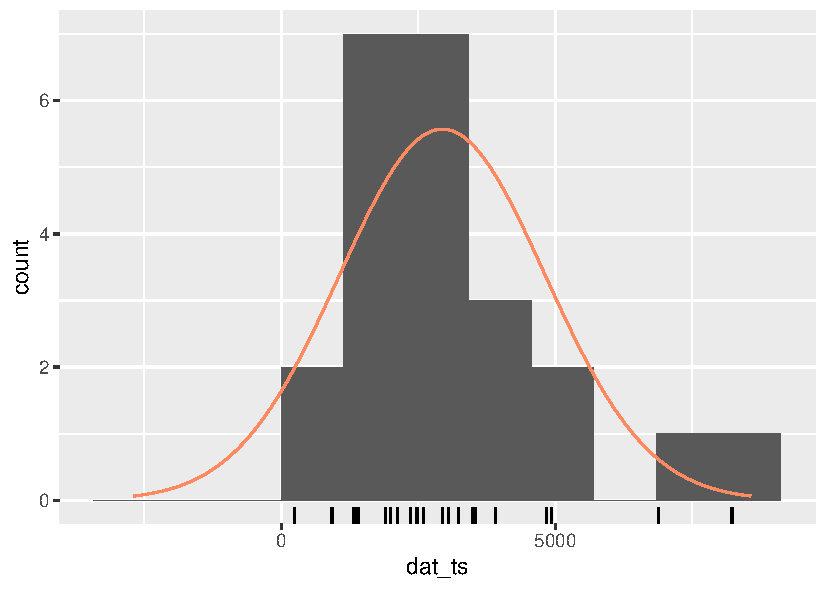
\includegraphics[width=\linewidth]{Ireland-residuals.pdf} \label{fig:ireland-residuals}
\endminipage\hfill
\minipage{0.33\textwidth}
  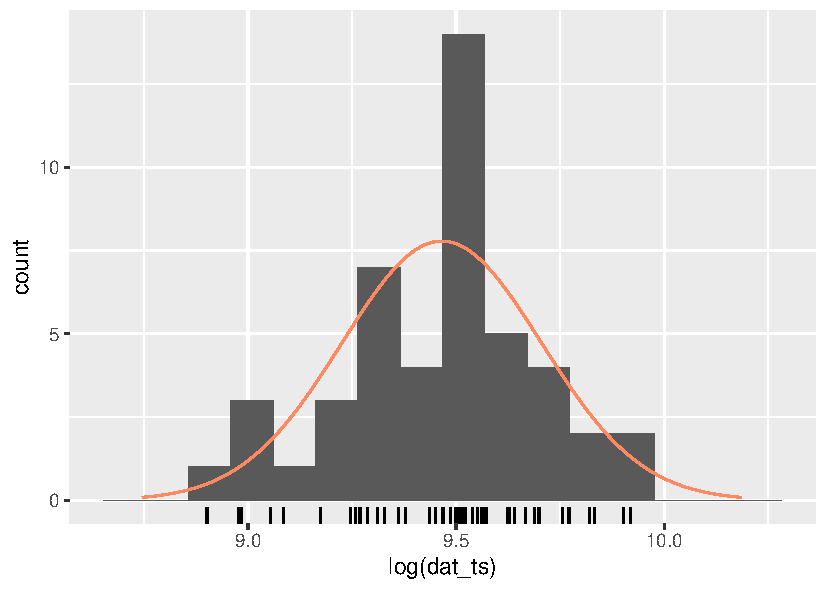
\includegraphics[width=\linewidth]{Italy-residuals.pdf} \label{fig:italy-residuals}
\endminipage\hfill
\minipage{0.33\textwidth}
  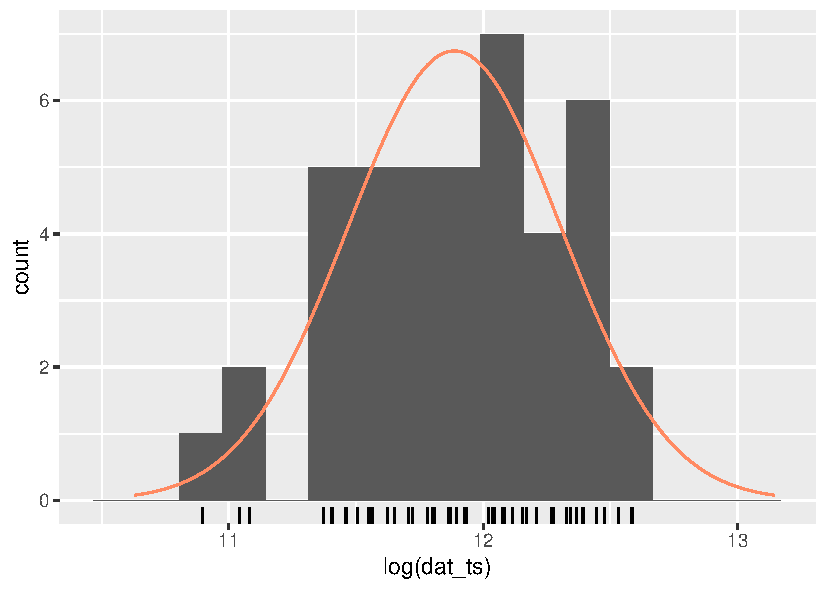
\includegraphics[width=\linewidth]{United States-residuals.pdf} \label{fig:usa-residuals}
\endminipage\hfill
\caption{Normality checks, Ireland, Italy and United States}
\end{figure}

\subsection{Holt-Winters’ seasonal method}

The Holt-Winters seasonal exponential smoothing algorithm models three aspects of the time series: the average value at different levels, the trend over time, and any seasonality.

\subsubsection{Definitions and Theory}

\begin{figure}[H]
\centering
\begin{tcolorbox}[width=.65\textwidth]%

Suppose there are $N$ observations.

Initial step:

$\left|\begin{array}{l}
L_s = \frac1s \sum_{i=1}^s x_i \\
b_s = \frac1s \left[\frac{x_{s+1}-x_1}{s}+\frac{x_{s+2}-x_2}{s}+\dots+\frac{x_{2s}-x_s}{s}\right]\\
S_n  = x_n-L_s, \ n=1,\dots,s
\end{array}\right.$

and choose parameters $0\leq\alpha\leq1,\ 0\leq\beta\leq1$ and $0\leq\gamma\leq1$

Then compute for $s<n\leq N$:

$\left|\begin{array}{lll}
\text{Level} &       L_n & = \alpha (x_n-S_{n-s})+(1-\alpha)(L_{n-1}+b_{n-1})\\
\text{Trend} &      b_n & = \beta(L_n-L_{n-1})+(1-\beta)b_{n-1}\\
\text{Seasonal} & S_n & = \gamma (x_n-L_n) + (1-\gamma)S_{n-s}\\
\text{Forecast} & F_{n+1} & = L_n+b_n+S_{n+1-s}
\end{array}\right.$
For subsequent observations,

$F_{N+k}=L_N+k\cdot b_N+S_{N+k-s}$
\label{SHWx}
\end{tcolorbox}
\caption{Seasonal Holt-Winters' Additive Model Algorithm (denoted SHW$_{+}$)}
\end{figure}

The parameters $\alpha,\beta,\gamma$ are selected using Maximum Likelihood Estimation.

\subsubsection{Implementation in R}

\begin{lstlisting}[breaklines = true, escapeinside=||, tabsize = 4, caption = {Algorithm for HoltWinters Model}]
#lambda=0 ensures values stay positive
hwfcst     <- forecast::hw(dat_ts, h = forecastlen, seasonal = hwmethod, lambda = 0) |\Suppressnumber|
...
...
...|\Reactivatenumber|
plots[["hw"]]  <- plot_hw(countrydat, modeldat, cols, labs)
\end{lstlisting}

\subsubsection{Plots}

We see that the additive seasonal method is a better choice for both model fit and confidence interval size.

\begin{figure}[H]
\begin{center}
\minipage{0.98\textwidth}
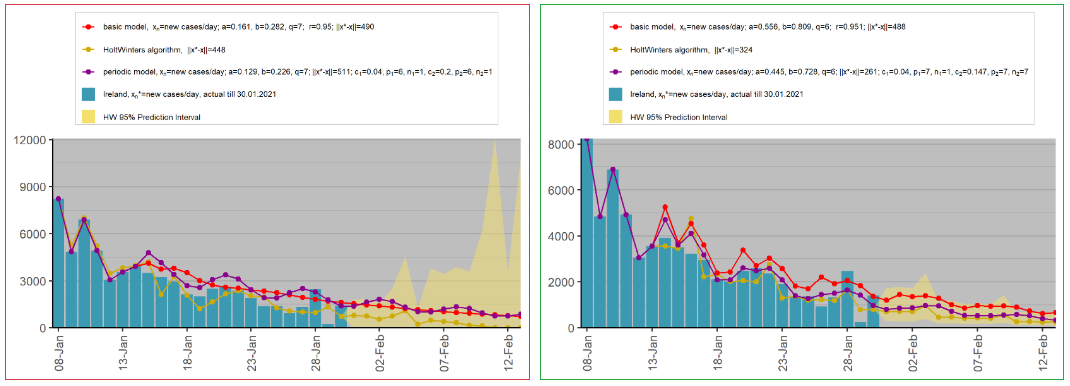
\includegraphics[width=0.9\linewidth]{hwaddmultcompare.png}
\endminipage\hfill
\caption{Comparison of HoltWinters multiplicative (left) and additive (right) algorithms}
\end{center}
\end{figure}

\begin{figure}[H]
\minipage{0.48\textwidth}
  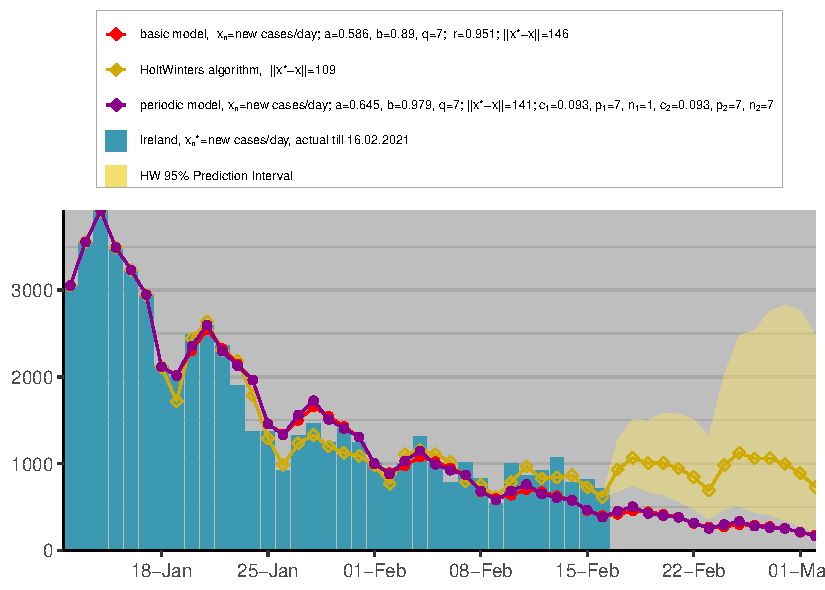
\includegraphics[width=\linewidth]{Ireland-hw.pdf} \label{fig:ireland-hw}
\endminipage\hfill
\minipage{0.48\textwidth}
  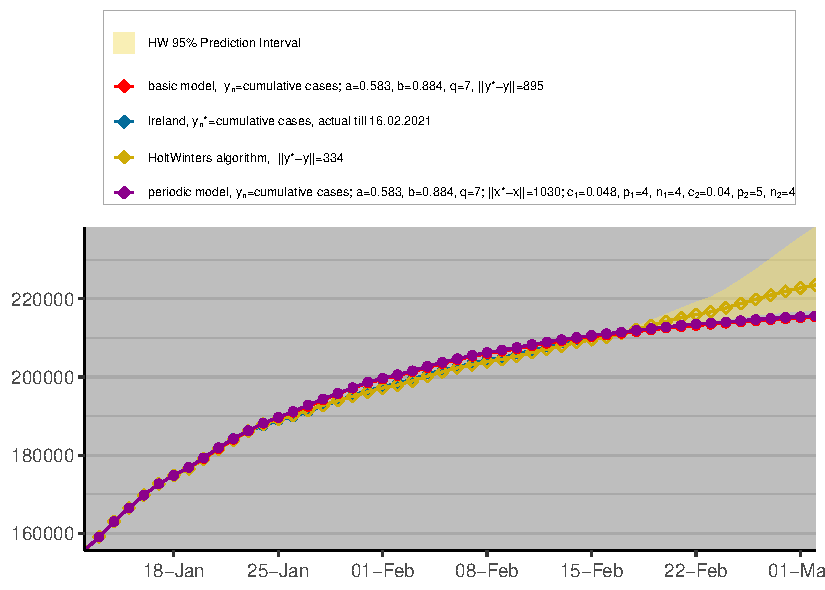
\includegraphics[width=\linewidth]{Ireland-hwy.pdf} \label{fig:ireland-hwy}
\endminipage
\caption{HoltWinters model, Ireland}
\end{figure}

\begin{figure}[H]
\minipage{0.48\textwidth}
  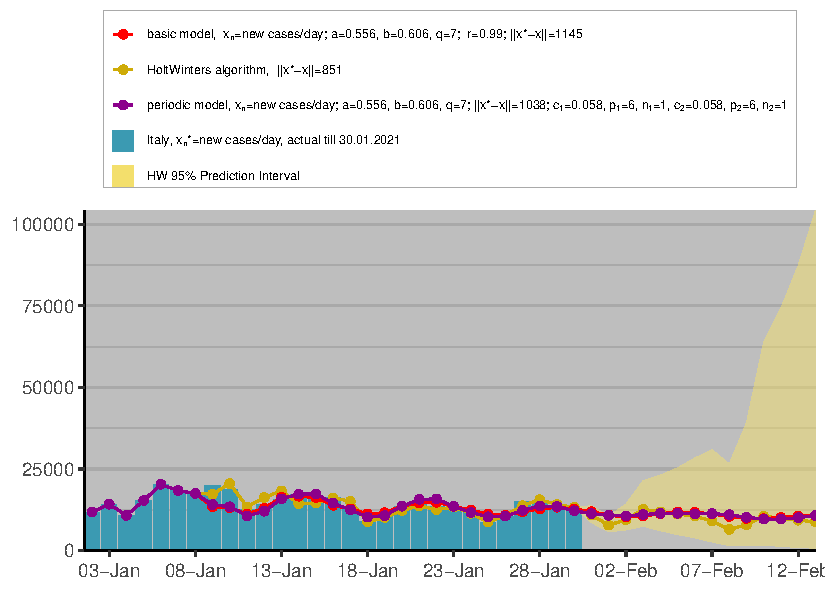
\includegraphics[width=\linewidth]{Italy-hw.pdf} \label{fig:italy-hw}
\endminipage\hfill
\minipage{0.48\textwidth}
  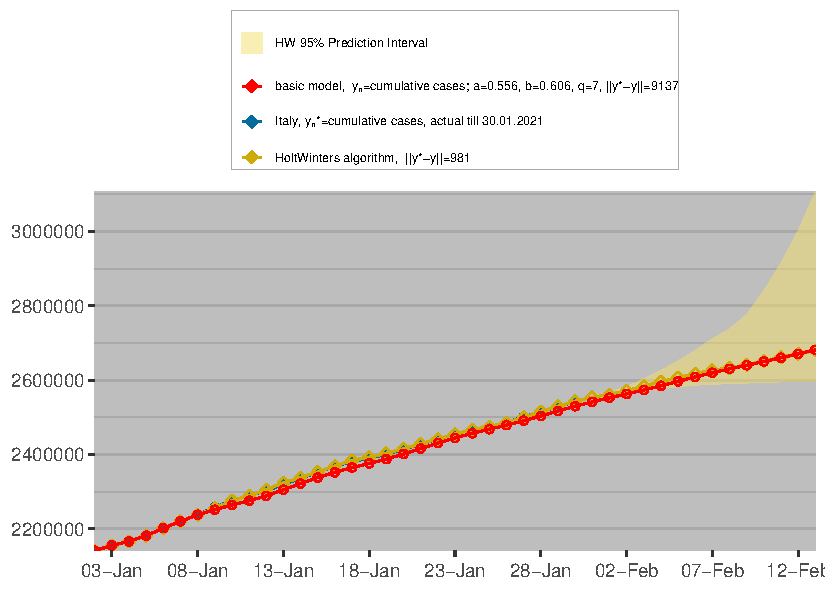
\includegraphics[width=\linewidth]{Italy-hwy.pdf} \label{fig:italy-hwy}
\endminipage
\caption{HoltWinters model, Italy}
\end{figure}

\begin{figure}[H]
\minipage{0.48\textwidth}
  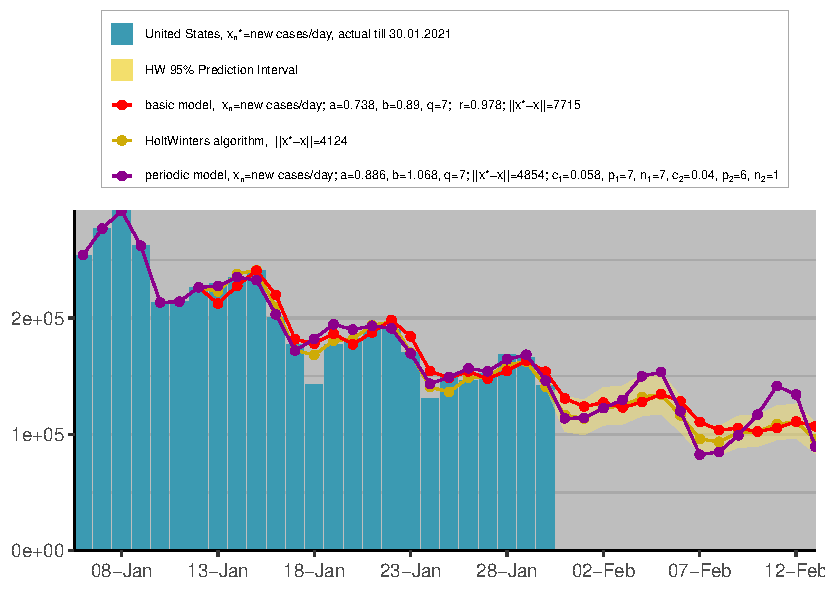
\includegraphics[width=\linewidth]{United States-hw.pdf} \label{fig:usa-hw}
\endminipage\hfill
\minipage{0.48\textwidth}
  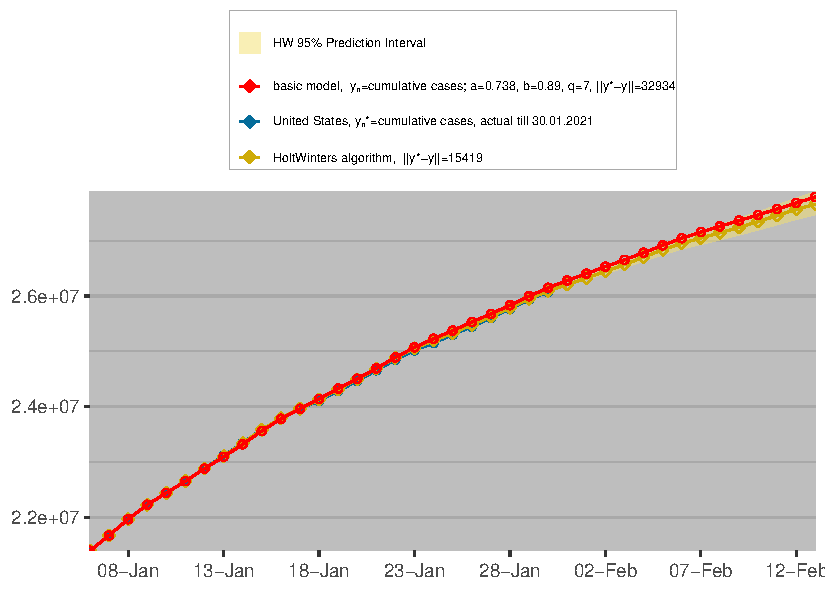
\includegraphics[width=\linewidth]{United States-hwy.pdf} \label{fig:usa-hwy}
\endminipage
\caption{HoltWinters model, United States}
\end{figure}

\subsection{ARIMA models}

\subsubsection{Definitions and Theory}

\begin{definition}
The \textit{backshift operator} $B$ is a function on a time series $\left(x_n\right)_{n\geq1}$ such that $Bx_n=x_{n-1}$ and more genrerally:

$$B^k x_n= x_{n-k},\quad n>k$$

And similarly for the independent errors $\eps_n$:

$$B^k \eps_n= \eps_{n-k},\quad n>k$$
\end{definition}

We must first define the each component of a non-seasonal ARIMA model (suitable for time series with a trend).

\begin{itemize}
\item An $AR(p)$ model, or an autoregressive model of order $p$ of a time series $x_1,\dots,x_N$ states that each $x_n$ is a \textit{linear function} of $x_{n-p},x_{n-p+1},\dots,x_{n-1}$ and an error term, i.e.
$$x_n= \phi_0+\phi_1 x_{n-1}+\phi_2 x_{n-2} +\dots + \phi_p x_{n-p}+\eps_n,\quad n>p,\quad \eps_n\sim N(0,\sigma^2)$$

Where there are constraints on the $\phi_0,\phi_1,\dots,\phi_p\in \mathbb{R}$

We can simplify using the backshift operator $B$:

\begin{align}
x_n
&= \phi_0+\phi_1 Bx_n+\phi_2 B^2x_n +\dots + \phi_p B^px_n +\eps_n\nonumber \\
&= \phi_0+\left(\phi_1 B+\phi_2 B^2 +\dots + \phi_p B^p\right)x_n +\eps_n
\end{align}

\item An $MA(k)$ model, or a moving average model of order $q$ of a time series $x_1,\dots,x_N$ states that each $x_n$ is a \textit{linear function} of the $q$ previous errors $\eps_{n-k},\eps_{n-k+1},\dots,\eps_{n-1}$, plus the current error $\eps_n$, i.e. 
$$x_n= \psi_0-\psi_1 \eps_{n-1}-\psi_2 \eps_{n-2} -\dots - \psi_k \eps_{n-k}+\eps_n,\quad n>p$$

By convention we use minus signs in the coefficients $\psi_1,\dots,\psi_k$
We can simplify using the backshift operator $B$:

\begin{align}
x_n
&= \psi_0-\psi_1 B\eps_n-\psi_2 B^2\eps_n -\dots - \psi_k B^k\eps_n + \eps_n \nonumber \\
&= \psi_0+\left(1-\psi_1 B-\psi_2 B^2 +\dots - \psi_k B^k\right)\eps_n 
\end{align}

\item The first order differencing of the time series, $I(1)$, is evalueated as 

\begin{align}
x_n'
&=x_n-x_{n-1}\nonumber \\
&=x_n-Bx_n \nonumber \\
&=\left(1-B\right)x_n
\end{align}

More generally, the differencing of order $d$, denoted $I(d)$ is 
$$(1-B)^d x_n$$

This only affects the $x_n$ (although constants are differenced to zero) and the errors $\eps_n$ are unchanged.
\end{itemize}

Therefore, an ARIMA$(p,d,k)$ model can be evaluated by combining the $AR(p),\ I(d)$ and $MA(k)$

\begin{align}
(1-B)^d x_n
&= \phi_0+(1-B)^d\left(\phi_1 B+\phi_2 B^2 +\dots + \phi_p B^p\right)x_n +
\psi_0+\left(\psi_1 B+\psi_2 B^2 +\dots + \psi_k B^k\right)\eps_n \nonumber 
\end{align}

\begin{align}
(1-B)^d x_n + (1-B)^d\left(-\phi_1 B-\phi_2 B^2 -\dots - \phi_p B^p\right)x_n
&= \phi_0 + \psi_0+\left(1-\psi_1 B-\psi_2 B^2 +\dots - \psi_k B^k\right)\eps_n  \nonumber \\
(1-B)^d\left(1-\phi_1 B-\phi_2 B^2 -\dots - \phi_p B^p\right)x_n
&=c+\left(1-\psi_1 B-\psi_2 B^2 +\dots - \psi_k B^k\right)\eps_n  \nonumber \\
\end{align}

where $c= \phi_0 + \psi_0$ (it is zero if $d\geq1$).

We also need the seasonal components for an ARIMA$(p,d,k)(P,D,K)_s$ 

Suppose a time series $x_n$ has period $s$ (seasonal pattern every $s$ values)
\begin{itemize}

\item An $AR(P)_s$ model, or a seasonal autoregressive model of order $P$ of a time series $x_1,\dots,x_N$ states that each $x_n$ is a \textit{linear function} of $x_{n-Ps},x_{n-(P-1)s},\dots,x_{n-s}$ and an error term, i.e. 
$$x_n= \beta_0+\beta_1 x_{n-s}+\beta_2 x_{n-2s} +\dots + \beta_P x_{n-Ps}+\eps_n$$

We can simplify using the backshift operator $B$:

\begin{align}
x_n &= \beta_0+\left(\beta_1 B^s+\beta_2 B^{2s} +\dots + \beta_P B^{Ps}\right)x_n
\end{align}

\item An $MA(K)_s$ model, or a seasonal moving average model of order $K$ of a time series $x_1,\dots,x_N$ states that each $x_n$ is a \textit{linear function} of the $K$ errors $\eps_{n-Ks},\eps_{n-(K-1)s},\dots,\eps_{n-s}$, plus the current error $\eps_n$, i.e. 
$$x_n= \gamma_0-\gamma_1 \eps_{n-s}-\gamma_2 \eps_{n-2s} -\dots - \gamma_K \eps_{n-Ks}+\eps_n$$

Again, by convention we use minus signs in the coefficients $\gamma_1,\dots,\gamma_K$

We can simplify using the backshift operator $B$:

\begin{align}
x_n
&= \gamma_0-\gamma_1 \eps_{n-s}-\gamma_2 \eps_{n-2s} -\dots - \gamma_K \eps_{n-Ks}+\eps_n \nonumber \\
&= \gamma_0+\left(1-\gamma_1 B^s-\gamma_2 B^{2s} +\dots - \gamma_K B^{Ks}\right)\eps_n 
\end{align}

\item The first order seasonal differencing of the time series, $I_s(1)$, is evalueated as 

$$x_n-x_{n-s}=\left(1-B^s\right)x_n$$

More generally, the seasonal differencing of order $D$, denoted $I_s(D)$ is 

$$(1-B^s)^D x_n$$

The purpose of this is to make the time series  stationary in mean
\end{itemize}


Then we can similarly compose our seasonal components (with seasonal period $s$) with the previous ARIMA$(pd,k)$ to get the definition of an ARIMA$(p,d,k)(P,D,K)_s$ model

\begin{align}\label{eq:arima}
\underbrace{\left(1-\phi_1 B-\phi_2B^2-\dots-\phi_p B^p\right)}_{AR(p)}
\underbrace{\left(1-\beta_1 B^s-\beta_2B^{2s}-\dots-\beta_P B^{Ps}\right)}_{AR_s(P)} 
\underbrace{\left(1-B\right)^d}_{I(d)}\underbrace{\left(1-B^s\right)^D}_{I_s(D)}   x_n = \nonumber \\
 c+
\underbrace{\left(1-\psi_1 B-\psi_2B^2-\dots-\psi_k B^k\right)}_{MA(k)}
\underbrace{\left(1-\gamma_1 B^s-\gamma_2B^{2s}-\dots-\gamma_K B^{Ks}\right)}_{MA_s(K)} \eps_n
\end{align}

where the constant $c$ is some function of the constants $\phi_0,\psi_0,\beta_0$ and $\gamma_0$ 

The orders $p, d, k$ and $P,D,K$ are computed by analysing the correlation functions (ACF and PACF).

The $P+K+p + k + 1$ coefficients $c, \phi_1, \dots , \phi_p, \psi_1,\dots , \psi_k, \beta_1,\dots,\beta_P,\gamma_1,\dots,\gamma_K$ are computed using Maximum Likelihood Estimation.

Again, \eqref{eq:arima} can similarly be used to compute forecasted values $x_{N+1},\dots,x_{N+m}$.

\begin{nremark}
Most of the literature, for example  \cite{Hyndman-et-al-2018}, use $q$ for non-seasonal and $Q$ for seasonal Moving Average models. I am using $k$ and $K$ respectively to avoid confusion with $q$ in the mathematical models \label{eq:xnrecurr}.
\end{nremark}

\subsubsection{Implementation in R}

\begin{lstlisting}[breaklines = true, escapeinside=||, tabsize = 4, caption = {Algorithm for ARIMA Model}]
#lambda=0 ensures values stay positive
auto.fit <- auto.arima(dat_ts, lambda = 0) |\Suppressnumber|
...
...
...|\Reactivatenumber|
plots[["arima"]]   <- plot_arima(countrydat, modeldat, cols, labs)
\end{lstlisting}

\subsubsection{Plots}

\begin{figure}[H]
\minipage{0.48\textwidth}
  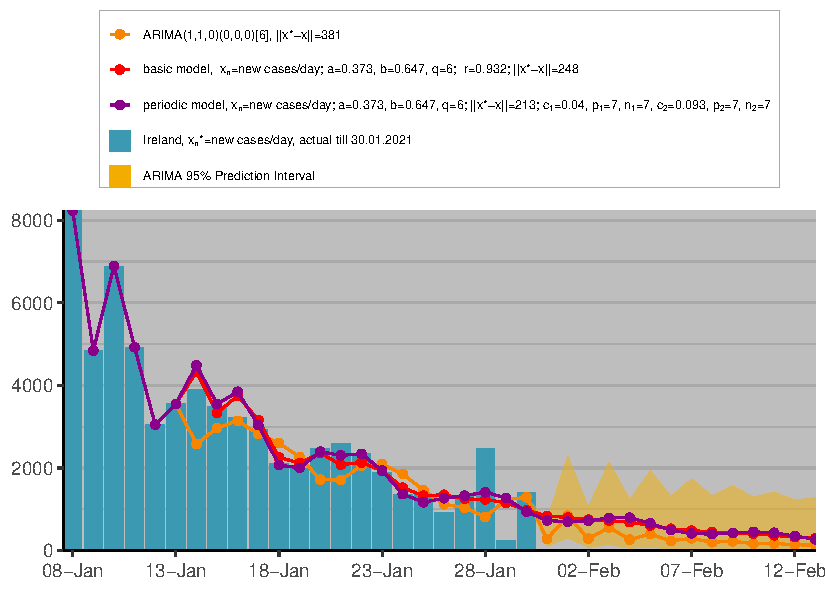
\includegraphics[width=\linewidth]{Ireland-arima.pdf} \label{fig:ireland-arima}
\endminipage\hfill
\minipage{0.48\textwidth}
  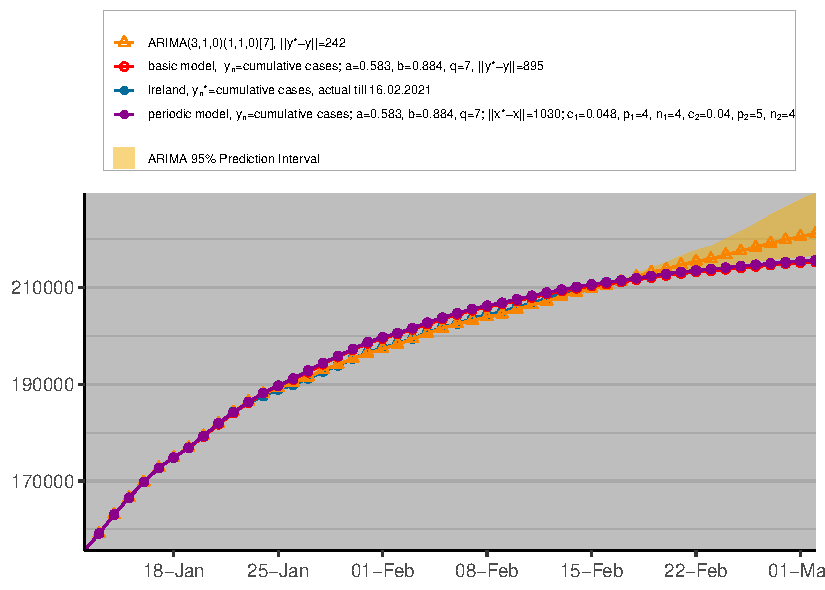
\includegraphics[width=\linewidth]{Ireland-arimay.pdf} \label{fig:ireland-arimay}
\endminipage
\caption{ARIMA model, Ireland}
\end{figure}

\begin{figure}[H]
\minipage{0.48\textwidth}
  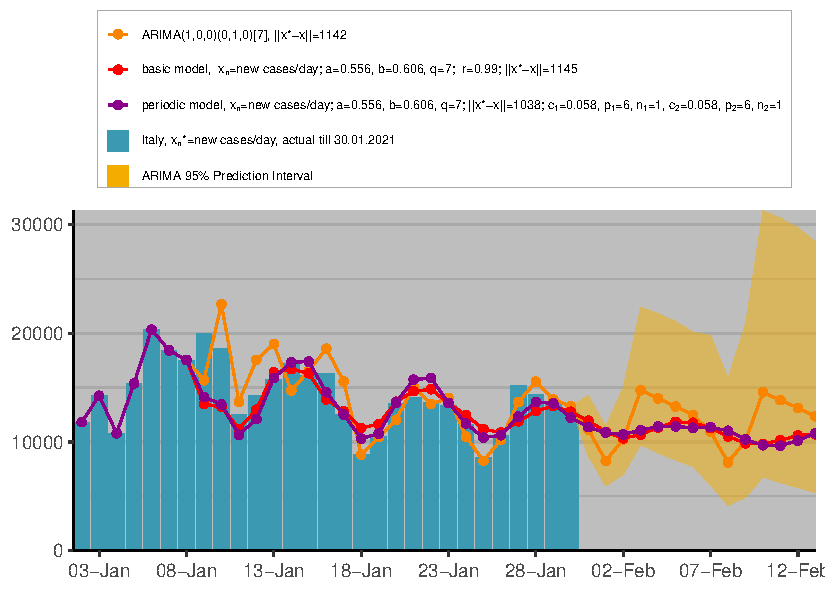
\includegraphics[width=\linewidth]{Italy-arima.pdf} \label{fig:italy-arima}
\endminipage\hfill
\minipage{0.48\textwidth}
  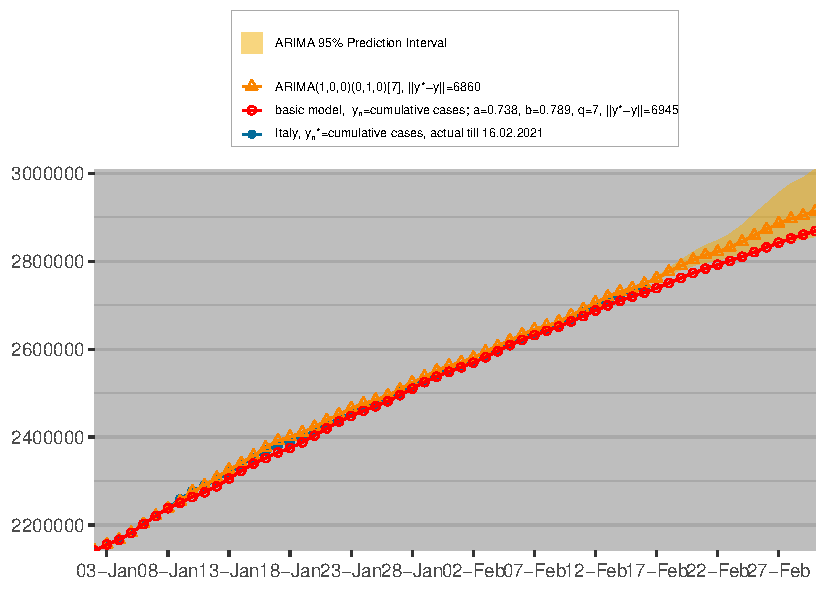
\includegraphics[width=\linewidth]{Italy-arimay.pdf} \label{fig:italy-arimay}
\endminipage
\caption{ARIMA model, Italy}
\end{figure}

\begin{figure}[H]
\minipage{0.48\textwidth}
  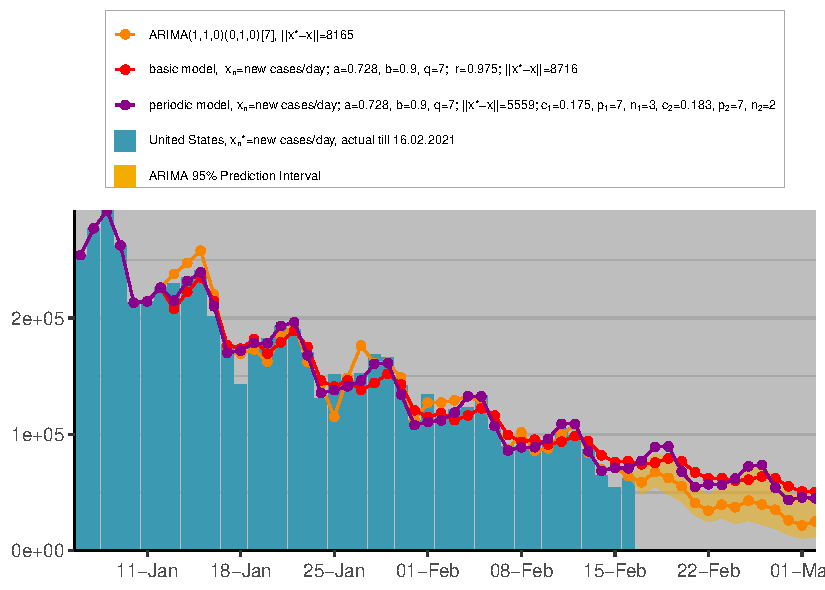
\includegraphics[width=\linewidth]{United States-arima.pdf} \label{fig:usa-arima}
\endminipage\hfill
\minipage{0.48\textwidth}
  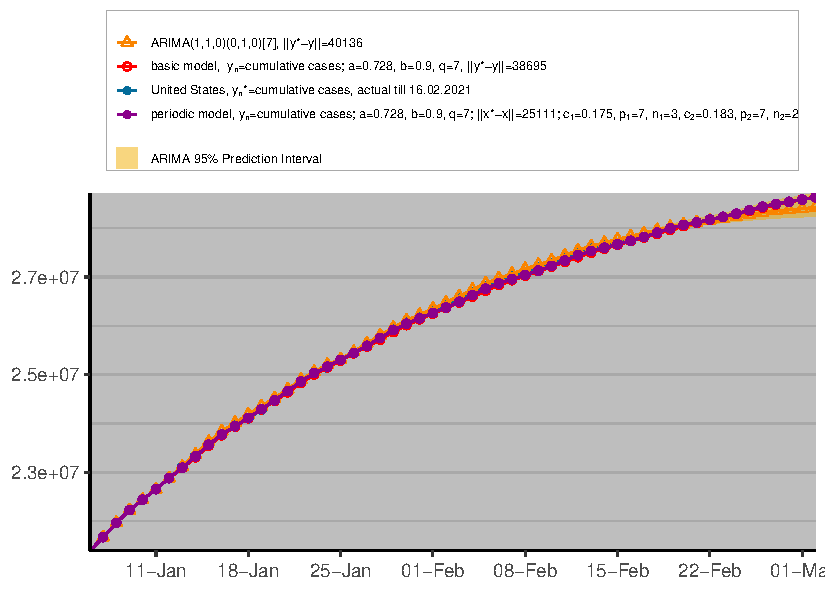
\includegraphics[width=\linewidth]{United States-arimay.pdf} \label{fig:usa-arimay}
\endminipage
\caption{ARIMA model, United States}
\end{figure}

\subsection{Neural network models}

An ARIMA$(p,0,0)$ has inputs $x_{n-1},\dots,x_{n-p}$ and parameters $\phi_{1},\dots,\phi_{p}$ in order to compute $x_n$ via a linear combination.

Similarly, an ARIMA$(p,0,0)(P,0,0)_s$ has inputs $x_{n-1},\dots,x_{n-p}, x_{n-s},\dots,x_{n-Ps}$ and parameters $\phi_{1},\dots,\phi_{p}, \beta_1,\dots,\beta_P$ in order to compute $x_n$ via another linear combination.

\begin{figure}[H]
\minipage{0.48\textwidth}
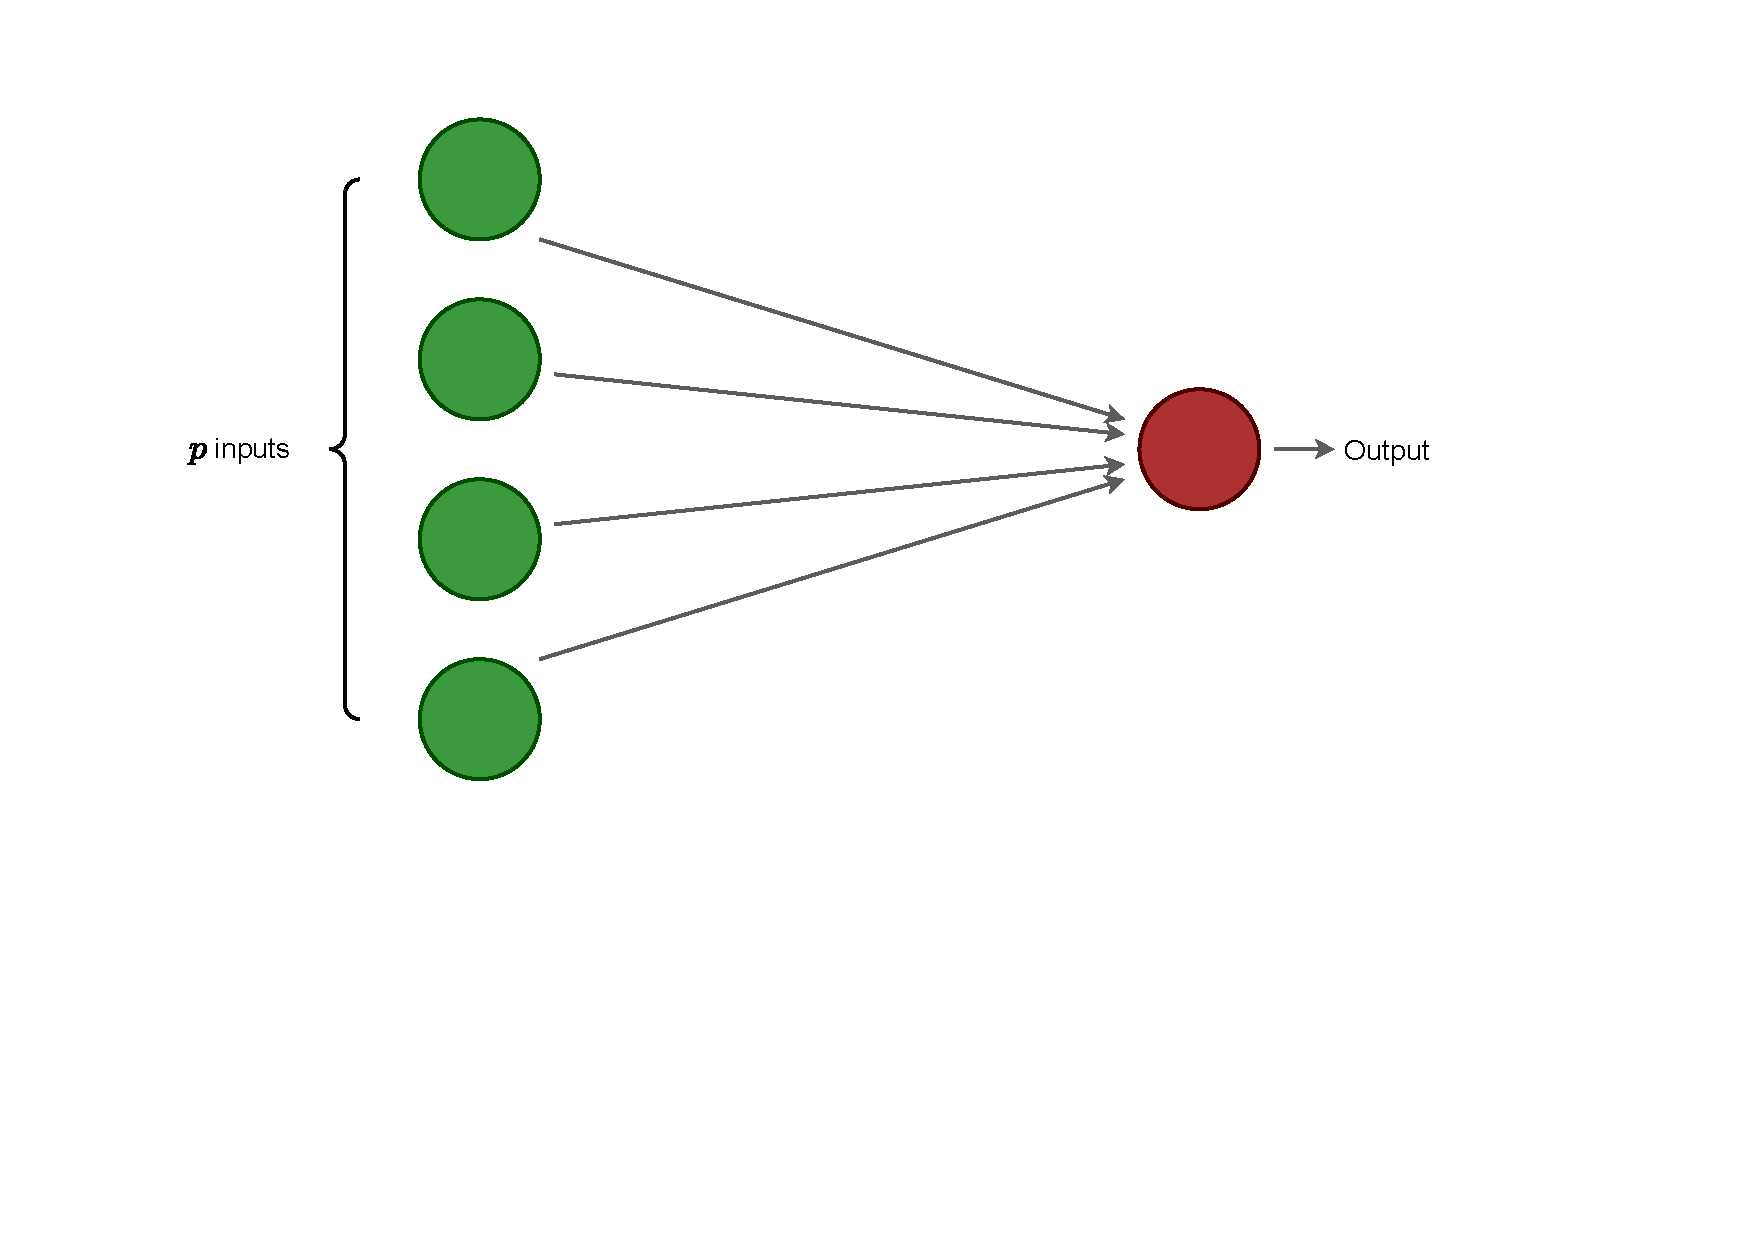
\includegraphics[width=0.9\textwidth]{NeuralNetNoHidden.pdf} 
\caption{A linear regression model, or ARIMA$(p,0,0)$ model.}
\label{fig:nnetnohidden}
\endminipage\hfill
\minipage{0.48\textwidth}
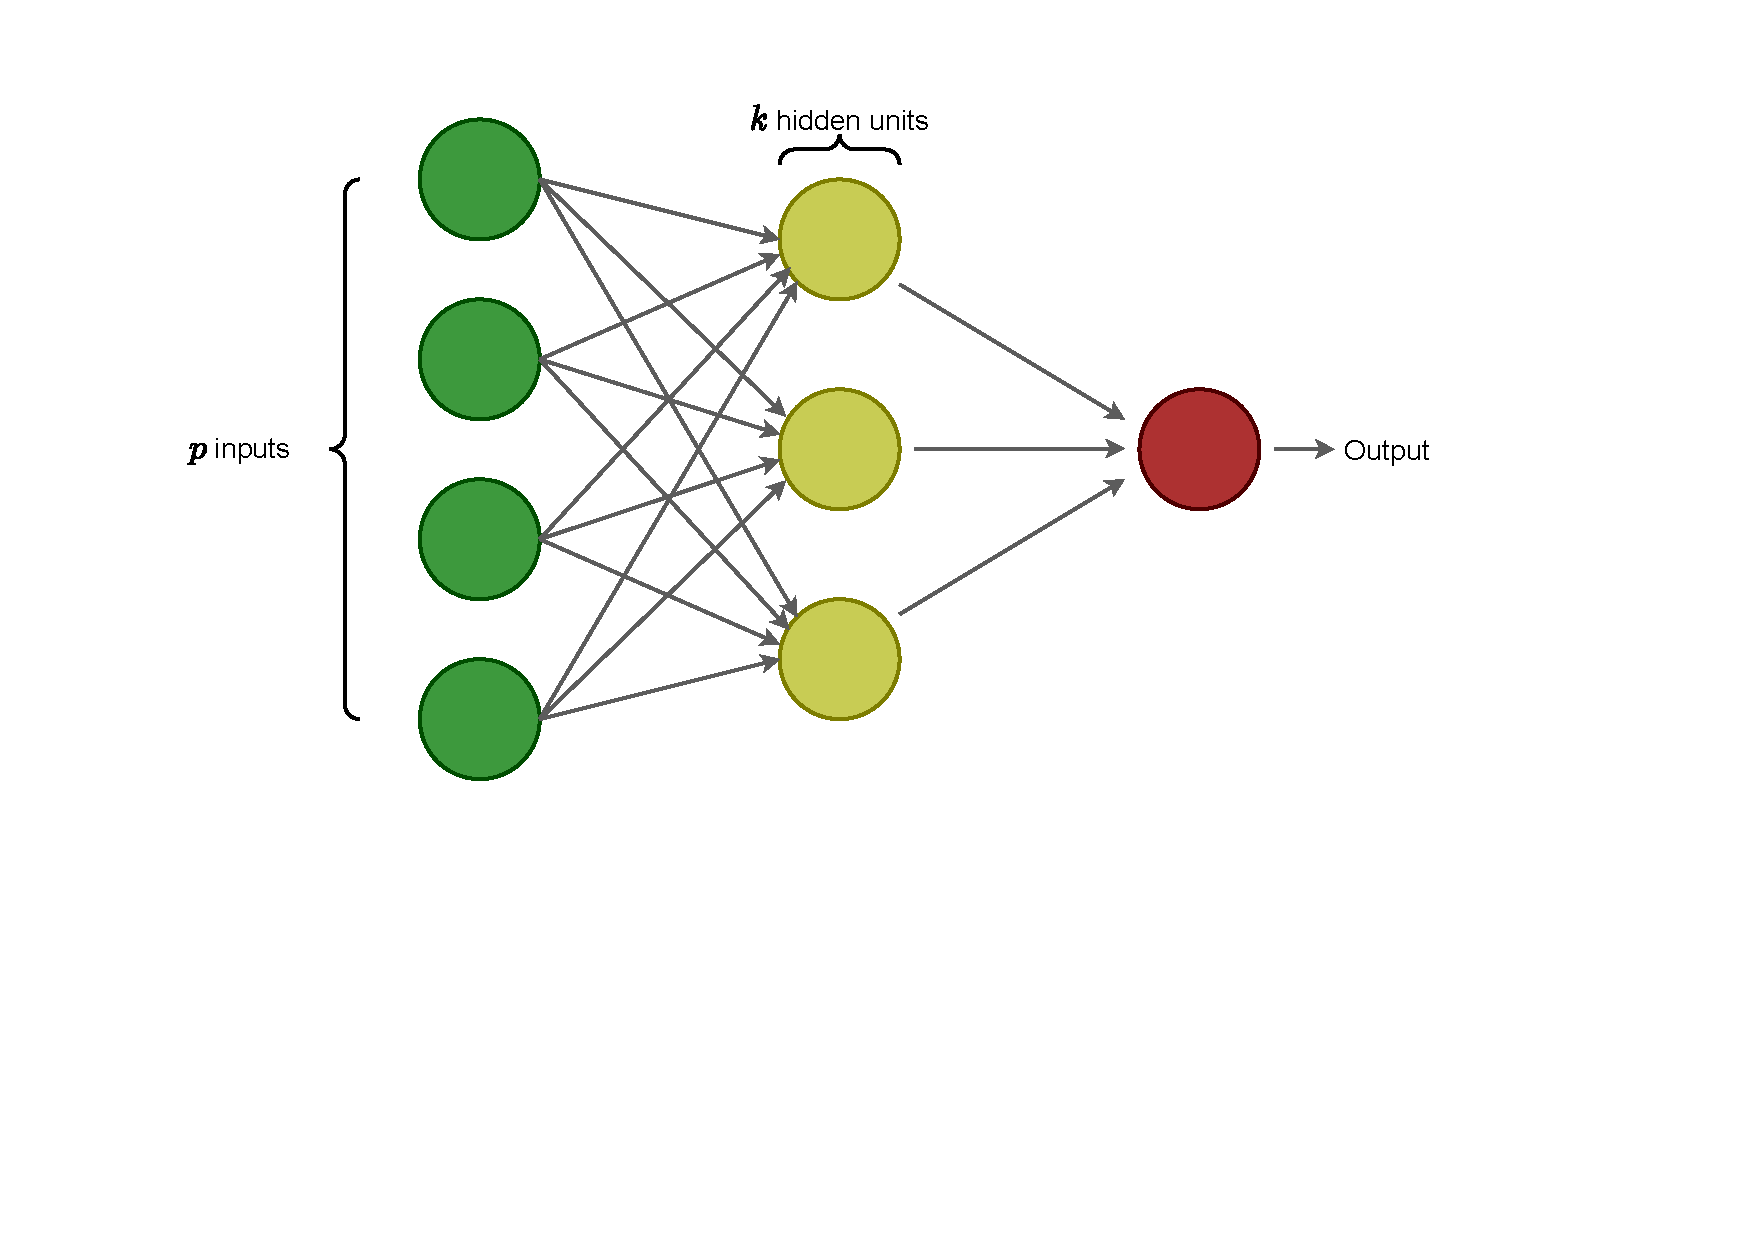
\includegraphics[width=0.9\textwidth]{NeuralNet.pdf}
\caption{A neural network with $p$ inputs and one hidden layer with $k$ hidden neurons.}
 \label{fig:nnet}
\endminipage
\end{figure}

With a Neiral Network Auroregressive model, a \textit{hidden layer} of $k$ inputs is introduced.

The model then becomes non-linear and allows for interactions between inputs (previous values in the time series).

The inputs to the hidden layer are then transformed using a sigmoid function

\begin{equation}\label{eq:sigmoid}
g(z)=\frac{1}{1+\exp(z)}
\end{equation}

The diagram \ref{fig:nnet} is a \textit{multilayer feed-forward network}, as each lconsecutive layer (left to right) of nodes takes inputs from the previous layer, adding complexity.

The \verb|forecast::nnetar()| function only allows for one layer to reduce the likelihood of overfiting of a univariate time series.

\subsubsection{Implementation in R}

\begin{lstlisting}[breaklines = true, escapeinside=||, tabsize = 4, caption = {Algorithm for NNAR Model}]
#lambda=0 ensures values stay positive
#size is the number of nodes in the hidden layer
nnfit   <- nnetar(dat_ts, p = auto.fit$arma[1], P = auto.fit$arma[3], size = nHidden, lambda = 0, repeats = 20, maxit = 50)  |\Suppressnumber|
...
...
...|\Reactivatenumber|
plots[["nn"]] <- plot_nn(countrydat, modeldat, cols, labs)
\end{lstlisting}

\subsubsection{Plots}

\begin{figure}[H]
\minipage{0.48\textwidth}
  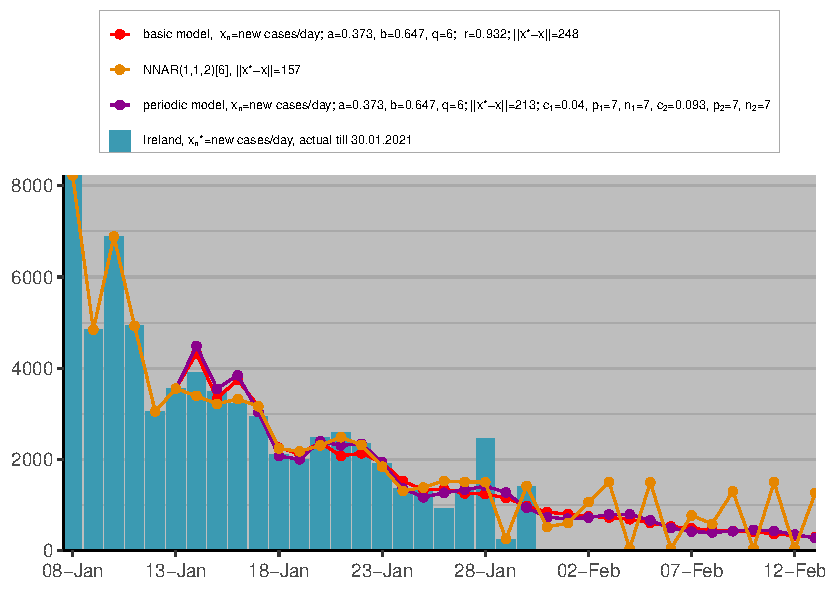
\includegraphics[width=\linewidth]{Ireland-nn.pdf} \label{fig:ireland-nn}
\endminipage\hfill
\minipage{0.48\textwidth}
  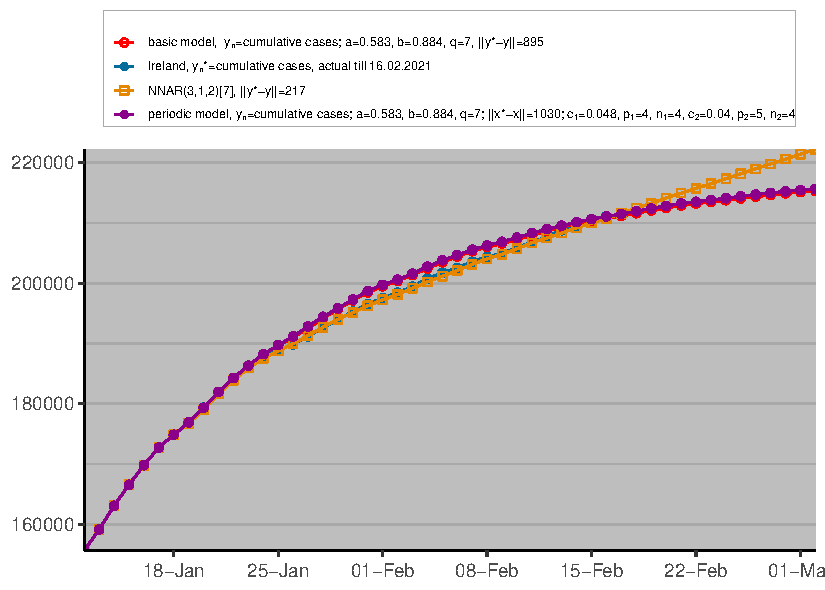
\includegraphics[width=\linewidth]{Ireland-nny.pdf} \label{fig:ireland-nny}
\endminipage
\caption{Neural Network Autoregression model, Ireland}
\end{figure}

\begin{figure}[H]
\minipage{0.48\textwidth}
  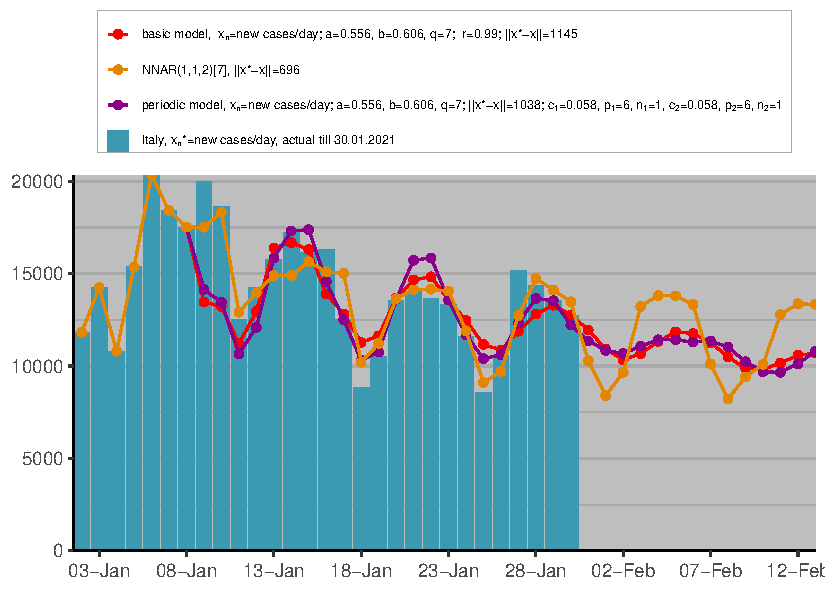
\includegraphics[width=\linewidth]{Italy-nn.pdf} \label{fig:italy-nn}
\endminipage\hfill
\minipage{0.48\textwidth}
  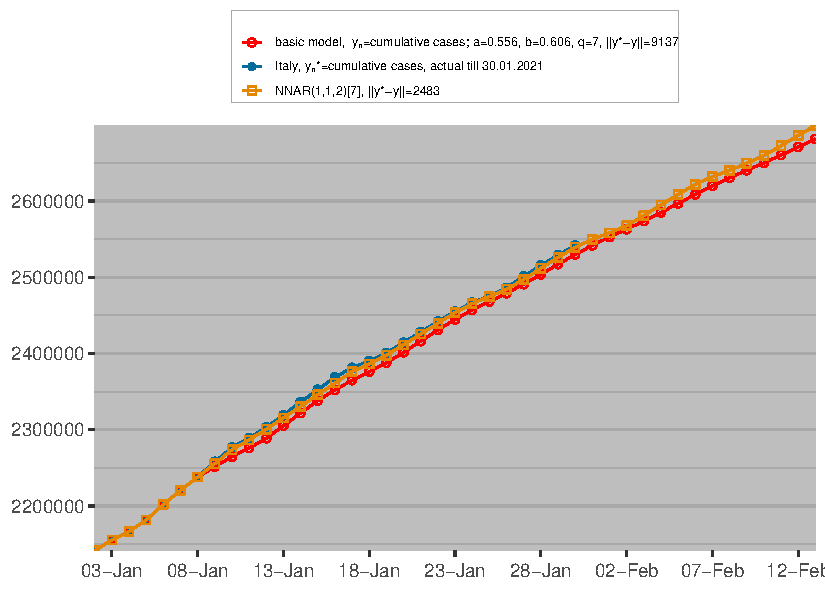
\includegraphics[width=\linewidth]{Italy-nny.pdf} \label{fig:italy-nny}
\endminipage
\caption{Neural Network Autoregression model, Italy}
\end{figure}

\begin{figure}[H]
\minipage{0.48\textwidth}
  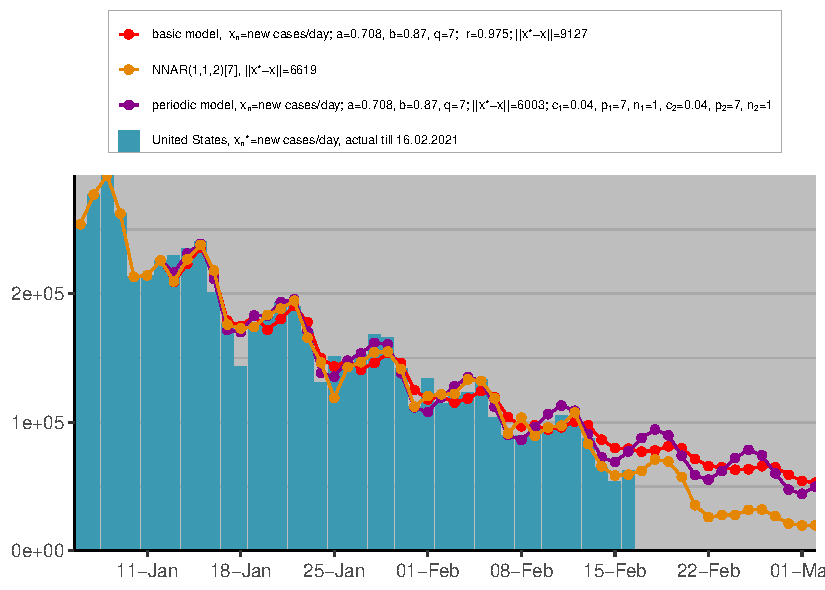
\includegraphics[width=\linewidth]{United States-nn.pdf} \label{fig:usa-nn}
\endminipage\hfill
\minipage{0.48\textwidth}
  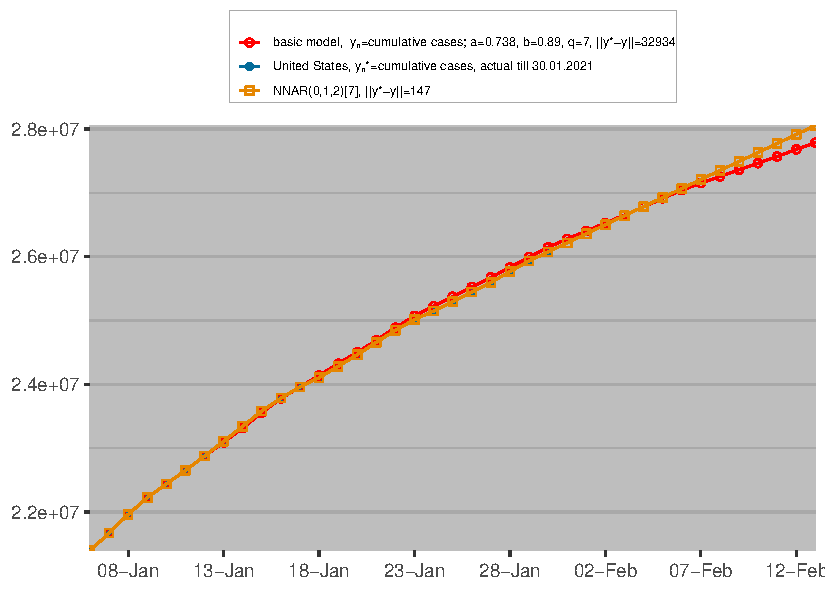
\includegraphics[width=\linewidth]{United States-nny.pdf} \label{fig:usa-nny}
\endminipage
\caption{Neural Network Autoregression model, United States}
\end{figure}
